% !TEX TS-program = pdflatex
% !TEX encoding = UTF-8 Unicode

\documentclass[11pt]{article} % use larger type; default would be 10pt

\usepackage{pgf}
\usepackage{tikz}
\usetikzlibrary{arrows,automata,shapes}
\usetikzlibrary{decorations.pathmorphing} % LATEX and plain TEX when using Tik Z

\usepackage[utf8]{inputenc} % set input encoding (not needed with XeLaTeX)

%%% PAGE DIMENSIONS
\usepackage{geometry} % to change the page dimensions
\geometry{a4paper} % or letterpaper (US) or a5paper or....
\geometry{margin=2cm} % for example, change the margins to 2 inches all round
% \geometry{landscape} % set up the page for landscape
%   read geometry.pdf for detailed page layout information

\usepackage{graphicx} % support the \includegraphics command and options
\usepackage{subcaption} % for subfigures

\usepackage{scrextend} % https://tex.stackexchange.com/questions/588/how-can-i-change-the-margins-for-only-part-of-the-text
\usepackage{color}
\definecolor{rowcolor}{rgb}{0.94, 0.97, 1.0}  % 1=weiß, 0=schwarz

% \usepackage[parfill]{parskip} % Activate to begin paragraphs with an empty line rather than an indent

%%% PACKAGES
\usepackage{booktabs} % for much better looking tables
\usepackage{array} % for better arrays (eg matrices) in maths
\usepackage{paralist} % very flexible & customisable lists (eg. enumerate/itemize, etc.)
\usepackage{verbatim} % adds environment for commenting out blocks of text & for better verbatim
%\usepackage{subfig} % make it possible to include more than one captioned figure/table in a single float
% These packages are all incorporated in the memoir class to one degree or another...
\usepackage{listings} % Absatz als Code formatieren
\usepackage{floatflt} % für floatingfigure

%%% HEADERS & FOOTERS
\usepackage{fancyhdr} % This should be set AFTER setting up the page geometry
\pagestyle{fancy} % options: empty , plain , fancy
\renewcommand{\headrulewidth}{0pt} % customise the layout...
\lhead{ZIMFLI QCoDeS Driver}\chead{}\rhead{\today}
\lfoot{Michael Wagener}\cfoot{\thepage}\rfoot{FZJ/ZEA-2}

%%% SECTION TITLE APPEARANCE
\usepackage{sectsty}
\allsectionsfont{\sffamily\mdseries\upshape} % (See the fntguide.pdf for font help)
% (This matches ConTeXt defaults)

%%% ToC (table of contents) APPEARANCE
\usepackage[nottoc,notlof,notlot]{tocbibind} % Put the bibliography in the ToC
\usepackage[titles,subfigure]{tocloft} % Alter the style of the Table of Contents
\renewcommand{\cftsecfont}{\rmfamily\mdseries\upshape}
\renewcommand{\cftsecpagefont}{\rmfamily\mdseries\upshape} % No bold!

\usepackage{longtable} % Tabellen über mehrere Seiten
\usepackage{multirow} % multirow/multicolumn
\usepackage{colortbl} % farbige Tabellenzellen
\setlength{\LTpre}{0pt}  % Remove whitespace befor and after longtables
\setlength{\LTpost}{0pt}
%\setlength{\LTleft}{1cm} % makes 1cm space at the left side of each longtable

\setlength{\tabcolsep}{1mm} % Setzt den Längenwert von {Abstand zwischen den Spalten einer Tabelle} auf den Wert 1mm
\setcounter{tocdepth}{2}  % Tiefe des Inhaltsverzeichnisses

\setlength{\parindent}{0em} % Damit die neuen Absätze nicht eingerückt werden

%%% END Article customizations

%%% The "real" document content comes below...

\title{QCoDeS driver for the Zurich Instruments Lock-In Amplifier (ZIMFLI)}
\author{Michael Wagener}

\begin{document}
\maketitle

\tableofcontents % toc anzeigen

%\ \\
\ \\

\begin{longtable}{|p{2.7cm}|p{2.6cm}|p{10.3cm}|}
%\caption{Document revision history} \\
%\hline\rowcolor{rowcolor}{\bf Date} & {\bf Author} & {\bf Short description} \\
\hline\rowcolor{rowcolor}{\bf Date} & {\bf Author} & {\bf Document revision history} \\
\endfirsthead
\hline
08. Mar. 2019 & M.Wagener & First edit phase. \\ \hline
14. Mar. 2019 & M.Wagener & Complete the parameter descriptions. \\ \hline
02. Jul. 2019 & M.Wagener & Describe the simulation. \\ \hline
17. Jul. 2019 & M.Wagener & Describe the Sweeper. \\ \hline
23. Jul. 2019 & M.Wagener & Describe test scripts \\ \hline
\end{longtable}


\clearpage

%%%
\section{Informations}

The Zurich Instruments Lock-In Amplifier (later only ZIMFLI) will be used in the QCoDeS Framework. Therefore a driver within this framework is needed. This is the user documentation for this driver describing in short form all parameters and some test scripts. \\[0.5em]
%
All tests are done with the ZIMFLI with the serial number 4039 in the ZEA-2. This device has the F5M option installed (means 5MHz insteand of 500kHz frequency range). This device was registered in our LAN during the tests. \\[0.5em]
%
All programming was done in the Spyder environment with Python 3.6.

\subsection{Git and directories}

This driver is inside the QCoDeS framework tree under {\bf Qcodes/qcodes/instrument\_drivers/ZI}. In the subdirectory {\bf TestScripts} are the scripts with all tests. They will be described later in this document. In the subdirectory {\bf Documentation} this documentation is located. The base of the QCoDeS framework used during the tests is the git branch \\
\centerline{\it https://github.com/qutech/Qcodes/tree/feature/qctoolkit-integration}
This driver is pushed to the git branch \\
\centerline{\it https://github.com/qutech/Qcodes/tree/feature/ziMFLI\_driver}


\subsection{Additional installations needed}

\begin{floatingfigure}[r]{0.42\textwidth}
\mbox{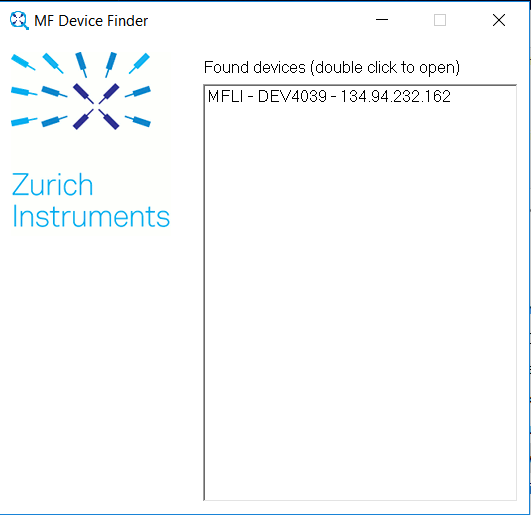
\includegraphics[width=0.4\textwidth]{ZI-DeviceFinder.png}}
\caption{ZI Device Finder}
\end{floatingfigure}
Don't forget to install the base driver from Zurich Instruments {\it https://www.zhinst.com/downloads}. Select the instrument {\it ``MFLI, MFIA''} and then the Software release version. Normally it is the best to leave the current version (for me it was 18.12). The first tests are done with the version 18.05 because the instrument has this version in its firmware. But the device runs also with the library-version 18.12. \\
Download and install the {\it Device Finder} for your Windows version or install the full packet {\it LabOne} for Windows or Linux. If you install the full packet, the documentation from ZI will also be installed.

You can connect the device to your USB port, the ZI software can install a special network driver for USB ports. After you connect the device to your network (or to your USB port), start the Device Finder and note the found device id.

{\it For your information: the Device Finder scans every few seconds the network for ZI devices. To avoid network traffic, close the Device Finder if you do not need it.}

Be sure that your computer is in the same subnet as the device. The Device Finder and later the driver cannot find the device if you use a VPN connection.

Then you have to install the Python package. From version 18.12 onwards you can start a shell and use the command
\begin{lstlisting}[frame=single]
pip install zhinst
\end{lstlisting}
All versions before have a separate download file on the ZI download page.

\clearpage


%%%
\section{General usage}

To use this driver, you have to import it and open the device. Be sure that you have the correct device id, it contains the serial number found with the {\it Device Finder}:

\begin{lstlisting}[frame=single, language=Python]
from qcodes.instrument_drivers.ZI.ZIMFLI import ZIMFLI
zidev = ZIMFLI( name='ZIMFLI', device_ID='DEV4039' )
\end{lstlisting}

During this open, the software searches for the device in the same subnet (or the USB). This will not work via VPN. The output in the test environment is:
\begin{lstlisting}[frame=single, language=Python]
Discovered device `dev4039`: MFLI with options F5M.
Creating an API session for device `dev4039` on `134.94.232.162`, `8004`
 with apilevel `6`.
\end{lstlisting}

In all following examples the variable {\bf zidev} is used as a reference to the device instance.

\ \\

After this you can access the device as decribed in detail later. As a first test you can get all version informations:
\begin{lstlisting}[frame=single, language=Python]
> import json
> print( json.dumps( zidev.version(), indent=4) )
{
    "DevType": "MFLI",
    "Options": "F5M",
    "Serial": "4039",
    "DevTime": "02.01.1970 10:41:25.265187",
    "Owner": "",
    "FPGARev": 52856,
    "DevFWRev": 53700,
    "BoardRev1": "1.4.G",
    "Copyright": "(c) 2008-2018 Zurich Instruments AG",
    "Dataserver": "ziDataServer",
    "ZI_FWRev": 0,
    "ZIRevision": 54618,
    "Version": "18.05"
}
\end{lstlisting}


\clearpage

%%%
\section{Base parameters}

The following parameters / subroutines are accessible directly from the main device instance.
% The names in square brackets after the function names are the Lock-In node names. This helps to convert the examples from the manual or the informations from the Web-GUI to the correct driver calls. The starting {\scriptsize /DEV.../} stands for the device ID, the {\scriptsize /n/} stands for an index starting at 0. All parameters without such notations are more complex functions.

\begin{itemize}
\item zidev.{\bf oscillator1\_freq}( {\it value} ) \\
	Reads (without a value) or writes the frequency of the oscillator. Before writing, the driver checks the valid range from 0 Hz to 500 kHz ( or 5 MHz if the F5M option is installed).
\item zidev.oscillator2\_freq( {\it value} ) \\
	Same for the second oscillator if the MD option is installed.
\item zidev.oscillator3\_freq( {\it value} ) \\
	Same for the third oscillator if the MD option is installed.
\item zidev.oscillator4\_freq( {\it value} ) \\
	Same for the fourth oscillator if the MD option is installed.

\item zidev.{\bf bufferedReader}( demod\_index, total\_time, dolog, copyFreq, copyPhase, copyDIO, copyTrigger, copyAuxin ) \\
	Read sample informations from the given demodulator for a given time as fast as possible (see Demodulator samplerate below) and returns it as a dict of arrays. The parameters are:
	\setlength{\LTleft}{1cm}
	\begin{longtable}{p{3.1cm}p{12cm}}
	demod\_index & index of demodulator channel (1,2) \\
	total\_time  & number of seconds for measurement, during this time the function is blocking \\
	dolog & Flag if this function print some informations during running (elapsed time and data length) \\
	copyFreq & Flag to copy the frequency data \\
	copyPhase & Flag to copy the phase data \\
	copyDIO & Flag to copy the digital I/O data \\
	copyTrigger & Flag to copy the trigger data \\
	copyAuxin & Flag to copy both auxin port data \\
	\multicolumn{2}{p{15cm}}{\it The copy flags can be set to False (default if omitted) to preserve memory usage. Set them to True to get more arrays in the resulting dict.} \\
	\end{longtable}
	\textbf{\textit{Return:}} a dict with dict\_keys(['timestamp', 'x', 'y', {\it 'frequency'}, {\it 'phase'}, {\it 'dio'}, {\it 'trigger'}, {\it 'auxin0'}, {\it 'auxin1'}, 'time', 'R', 'phi']).
	The fields `R' and `phi' are calculated from `x' and `y'. The italic fields must be switched on with the copy flags. All fields are arrays of the same length and contains the measured data. Execpt the field 'time' has the values:
%	\begin{longtable}{p{0.8cm}p{3.1cm}p{12cm}}
	\begin{longtable}{p{3.1cm}p{12cm}}
	'trigger' & 0 \\
	'dataloss' & False \\
	'blockloss' & False \\
	'ratechange' & False \\
	'invalidtimestamp' & False \\
	'mindelta' & 0 \\
	'clockbase' & 60000000.0  {\it this is used to calculate the correct time from the timestamps} \\
	\end{longtable}

\item zidev.{\bf version}() \\
  	Read all possible version informations and returns them as a dict. See the first example above.

\item zidev.{\bf getLastSampleTimestamp}() \\
	Get the time of last sample request. The return is a three value array:
	\setlength{\LTleft}{1.5cm}
	\begin{longtable}{p{0.5cm}p{14.4cm}}
	 $[0]$ & the current system time in seconds from time.time(). \\
	 $[1]$ & the timestamp value of the device. \\
	 $[2]$ & the timestamp of the device divided by the clockbase to get seconds. The absolute value of the seconds is not relevant because there is no function to set the current time, but the differences are useful. \\
	\end{longtable}

\item zidev.{\bf close}() \\
	Override the base class close function to perform a local cleanup and to disconnect from the device.

\item zidev.{\bf Scope} \\
  	Submodule for the scope functionality. This is under development.

\item zidev.{\bf Sweep} \\
	Submodule for the Sweep functionality. See chapter \ref{lblsweep} on page \pageref{lblsweep}.
\item zidev.{\bf add\_signal\_to\_sweeper}(demodulator, attribute) \\
	Helper function to add a signal to the output of the sweeper get function. See \ref{lblsweep}.
\item zidev.{\bf remove\_signal\_from\_sweeper}(demodulator, attribute) \\
	Helper function to remove a signal from the output of the sweeper get function. See \ref{lblsweep}.
\item zidev.{\bf print\_sweeper\_settings}() \\
	Helper function to print all settings of the sweep. See \ref{lblsweep}.

\item zidev.{\bf getClockbase}() \\
	Value of the clockbase to calculate the correct time from the timestamps.
	%%% --> Beispiel ?

\item zidev.{\bf getOptions}() \\
	Option string from the device. This string is read at the start of the driver from the device to apply the correct parameters and values.
  
\end{itemize}


%%%
\section{Submodules}

In this section all implemented submodules for this device are described. For each submodule all available parameters are listed with a short description.

\subsection{Demodulator}
The Lock-In-Amplifier has two demodulator channels. Not all parameters are accessible for the second channel. If the MD option is installed, there are four channels available. The submodules are named {\bf demod1} and {\bf demod2}, \small{with the MD option up to demod4}. The class is {\it DemodulatorChannel} with the following parameters:
	\begin{itemize}
	\item {\bf bypass}: Allows to bypass the demodulator low-pass filter, thus increasing the bandwidth.
	\item {\bf frequency}: {\it (ReadOnly)} Indicates the frequency used for demodulation and for output generation. The demodulation frequency is calculated with oscillator frequency times the harmonic factor. When the MOD option is used, linear combinations of oscillator frequencies including the harmonic factors define the demodulation frequencies.
	\item {\bf order}: Selects the filter roll off. Allowed Values:
	\setlength{\LTleft}{1.5cm}
	\begin{longtable}{p{1cm}p{14cm}}
	1 & 1st order filter 6 dB/oct \\
	2 & 2nd order filter 12 dB/oct \\
	3 & 3rd order filter 18 dB/oct \\
	4 & 4th order filter 24 dB/oct \\
	5 & 5th order filter 30 dB/oct \\
	6 & 6th order filter 36 dB/oct \\
	7 & 7th order filter 42 dB/oct \\
	8 & 8th order filter 48 dB/oct \\
	\end{longtable}
	\item {\bf harmonic}: Multiplies the demodulator's reference frequency by an integer factor. If the demodulator is used as a phase detector in external reference mode (PLL), the effect is that the internal oscillator locks to the external frequency divided by the integer factor.
	\item {\bf oscselect}: Connects the demodulator with the supplied oscillator. Number of available oscillators depends on the installed options. Is a number between 0 and the number of oscillators -1.
	\item {\bf phaseadjust}: Adjust the demodulator phase automatically in order to read 0 degrees.
	\item {\bf phaseshift}: Phase shift applied to the reference input of the demodulator. The value is clipped by the device to -180 .. +180 degrees.
	\item {\bf timeconstant}: Sets the integration time constant or in other words, the cutoff frequency of the demodulator low pass filter.
	\item {\bf samplerate}$^{(*)}$: Defines the demodulator sampling rate, the number of samples that are sent to the host computer per second. A rate of about 7-10 higher as compared to the filter bandwidth usually provides sufficient aliasing suppression. This is also the rate of data received by LabOne Data Server and saved to the computer hard disk. This setting has no impact on the sample rate on the auxiliary outputs connectors. {\it Note: the value inserted by the user may be approximated to the nearest value supported by the instrument.}
	\item {\bf sample}$^{(*)}$: {\it (ReadOnly)} Returns a dict with streamed demodulator samples with sample interval defined by the demodulator data rate. See note below. The dict contains the following entries:
	\setlength{\LTleft}{0.9cm}
	\begin{longtable}{p{3.1cm}p{12.7cm}}
	'timestamp' & array of uint64 with the internal timestamp of the measurement. Divide this by zidev.clockbase to get the real time in seconds. \\
	'x' & array of double with the x part of the demodulated cartesian coordinates \\
	'y' & array of double with the y part of the demodulated cartesian coordinates \\
	'frequency' & array of double with the current frequency of the oscillator \\
	'phase' & array of double with the angle of the demodulator polar coordinates \\
	'dio' & array of uint32 with the values of the digital inputs \\
	'trigger' & array of uint32 \\
	'auxin0' & array of double with the voltage of the first auxiliary input \\
	'auxin1' & array of double with the voltage of the second auxiliary input \\
	'R' & array of double with the calculated radius of the demodulated polar coordinates, see note below. \\
	'phi' & array of double with the calculated angle of the demodulated polar coordinates, see note below. \\
	\end{longtable}
	\item {\bf sinc}: Enables the sinc filter. When the filter bandwidth is comparable to or larger than the demodulation frequency, the demodulator output may contain frequency components at the frequency of demodulation and its higher harmonics. The sinc is an additional filter that attenuates these unwanted components in the demodulator output. Possible values are: 'ON', 'OFF'.
	\item {\bf signalinput}: Selects the input signal for the demodulator. Possible values: 'Sig In 1', 'Curr In 1', 'Trigger 1', 'Trigger 2', 'Aux Out 1', 'Aux Out 2', 'Aux Out 3', 'Aux Out 4', 'Aux In 1', 'Aux In 2', 'Constant input'.
	\item {\bf streaming}$^{(*)}$: Enables the data acquisition for the corresponding demodulator. Possible values are: `ON', `OFF'.
	\item {\bf trigger}$^{(*)}$: Selects the acquisition mode (i.e. triggering) or the demodulator. The possible values are:
	\setlength{\LTleft}{0.9cm}
	\begin{longtable}{p{3.1cm}p{12.7cm}}
	'Continuous' & demodulator data is continuously streamed to the host computer \\
	'Trigger in 1 Rise' & rising edge triggered \\
	'Trigger in 1 Fall' & falling edge triggered \\
	'Trigger in 1 Both' & triggering on both rising and falling edge \\
	'Trigger in 2 Rise' & rising edge triggered \\
	'Trigger in 2 Fall' & falling edge triggered \\
	'Trigger in 2 Both' & triggering on both rising and falling edge \\
	'Trigger in 1$\mid$2 Rise' & rising edge triggered on either input \\
	'Trigger in 1$\mid$2 Fall' & falling edge triggered on either input \\
	'Trigger in 1$\mid$2 Both' & triggering on both rising and falling edge or either trigger input \\
	'Trigger in 1 Low' & demodulator data is streamed to the host computer when the level is low (TTL) \\
	'Trigger in 1 High' & demodulator data is streamed to the host computer when the level is high (TTL) \\
	'Trigger in 2 Low' & demodulator data is streamed to the host computer when the level is low (TTL) \\
	'Trigger in 2 High' & demodulator data is streamed to the host computer when the level is high (TTL) \\
	'Trigger in 1$\mid$2 Low' & demodulator data is streamed to the host computer when either level is low (TTL) \\
	'Trigger in 1$\mid$2 High' & demodulator data is streamed to the host computer when either level is high (TTL) \\
	\end{longtable}
	\item {\bf x}: {\it (ReadOnly)} get sample of x coordinate. See note below.
	\item {\bf y}: {\it (ReadOnly)} get sample of y coordinate. See note below.
	\item {\bf R}: {\it (ReadOnly)} get sample of absolute value of x+y*i. See note below.
	\item {\bf phi}: {\it (ReadOnly)} get sample of angle of x+y*i. See note below.
	\item {\bf cfgTimeout}: stores the  used timeout in seconds for the readings of sample data (default 0.07). The valid range is from 0 to 1 second.
	\item[$^{(*)}$] all parameters marked with this are only accessible for channel 1 or, if the MD option is installed, also on other channels.
	\end{itemize}
	{\bf Note:} {\it The values of x and y are inside the sample dict, the values of R and phi are calculated. To have all values at the same measurement timestamp, the driver asks the device only if the last sample request is more than the cfgTimeout seconds ago.}


\subsection{Signal Input (Voltage)}
The Lock-In-Amplifier has one voltage sensitive input channel. The submodule is named {\bf signal\_in1}, the class is {\it SignalInputChannel} with the following parameters:
\begin{itemize}
\item {\bf autorange}: Automatic adjustment of the Range to about two times the maximum signal input amplitude measured over about 100 ms.
\item {\bf range}: Defines the gain of the analog input amplifier. The range should exceed the incoming signal by roughly a factor two including a potential DC offset. The instrument selects the next higher available range relative to a value inserted by the user. A suitable choice of this setting optimizes the accuracy and signal-to-noise ratio by ensuring that the full dynamic range of the input ADC is used.
\item {\bf float}: Switches the input between floating ('ON') and connected to ground ('OFF'). This setting applies both to the voltage and the current input. It is recommended to discharge the test device before connecting or to enable this setting only after the signal source has been connected to the Signal Input in grounded mode.
\item {\bf scaling}: Applies the given scaling factor to the input signal.
\item {\bf ac}: Defines the input coupling for the Signal Inputs. AC coupling ('ON') inserts a high-pass filter. 'OFF' means DC ccoupling.
\item {\bf impedance}: Switches the input impedance between 50 Ohm ('ON') and 10 M Ohm ('OFF').
\item {\bf diff}: Switches between single ended ('OFF', use only +V input) and differential ('ON', use both +V and -V inputs) measurements.
\item {\bf max}: Indicates the maximum measured value at the input.
\item {\bf min}: Indicates the minimum measured value at the input.
\item {\bf on}: Enables the signal input.
\item {\bf trigger}: Switches to the next appropriate input range such that the range fits best with the measured input signal amplitude.
\end{itemize}


\subsection{Signal Input (Current)}
The device has one current sensitive input channel. The submodule is named {\bf current\_in1}, the class is {\it CurrentInputChannel} with the following parameters:
\begin{itemize}
\item {\bf autorange}: Automatic adjustment of the Range to about two times the maximum signal input amplitude measured over about 100 ms.
\item {\bf range}: Defines the gain of the analog input amplifier. The range should exceed the incoming signal by roughly a factor two including a potential DC offset. The instrument selects the next higher available range relative to a value inserted by the user. A suitable choice of this setting optimizes the accuracy and signal-to-noise ratio by ensuring that the full dynamic range of the input ADC is used.
\item {\bf float}: Switches the input between floating ('ON') and connected to ground ('OFF'). This setting applies both to the voltage and the current input. It is recommended to discharge the test device before connecting or to enable this setting only after the signal source has been connected to the Signal Input in grounded mode.
\item {\bf scaling}: Applies the given scaling factor to the input signal.
\item {\bf max}: Indicates the maximum measured value at the input.
\item {\bf min}: Indicates the minimum measured value at the input.
\item {\bf on}: Enables the signal input.
\item {\bf trigger}: Switches to the next appropriate input range such that the range fits best with the measured input signal amplitude.
\end{itemize}


\subsection{Auxiliary Inputs}
The device has two auxiliary inputs. Because of the demodulator functionality the input values are only available as fields in the dict of the demodulator sample reading. The submodule is named {\bf aux\_in1}, the class is {\it AUXInputChannel} with the following parameters:
\begin{itemize}
\item {\bf averaging}: Defines the number of samples on the input to average as a power of two. Possible values are in the range [0, 16]. A value of 0 corresponds to the sampling rate of the auxiliary input's ADC.
\item {\bf sample}: This returns the same dict as the demodulator parameter sample.
\end{itemize}


\subsection{External reference}
The device has the capability to synchronize its internal oscillator used for demodulation with an external reference clock signal. The submodule is named {\bf extref1}, the class is {\it ExternalReferenceChannel} with the following parameters:
\begin{itemize}
\item {\bf signalin}: {\it (ReadOnly)} Indicates the input signal selection for the selected demodulator. Possible Values are 'Sig In 1', 'Curr In 1', `Trigger 1', 'Trigger 2', 'Aux Out 1', 'Aux Out 2', 'Aux Out 3', 'Aux Out 4', 'Aux In 1', 'Aux In 2', `Constant'. This value can be set with the {\it signalinput} parameter in the {\it demod1/2} module.
\item {\bf automode}: {\it (Only \underline{with} MD option installed)} This defines the type of automatic adaptation of parameters in the PID used for external reference. Allowed values are 'None', 'PID Auto', 'PID Low', 'PID High', 'PID All'.
\item {\bf bandwidth}: {\it (Only \underline{without} MD option installed)} This defines the bandwidth used for external reference. Allowed values are `None', `Low', `High'.
\item {\bf channel}: {\it (ReadOnly)} Indicates the demodulator connected to the extref channel.
\item {\bf enable}: Enables the external reference. Allowed Values are 'ON' and 'OFF'.
\item {\bf locked}: {\it (ReadOnly)} Indicates whether the external reference is locked.
\item {\bf oscselect}: {\it (ReadOnly)} Indicates which oscillator is being locked to the external reference.
\end{itemize}
In the following example the external reference is switched on, set to low bandwidth and the input is set to the auxiliary input 1:
% die Leerzeichen vor den # sind TABs damit die # übereinander stehen!
\begin{lstlisting}[frame=single, language=Python]
er = zidev.submodules['extref1']	# select submodule
er.enable('ON')				# switch external reference on
er.bandwidth('Low')			# select low bandwidth
dm2 = zidev.submodules['demod2']	# get another submodule
dm2.signalin('Aux In 1')		# select input for external reference
\end{lstlisting}


\subsection{Signal Output}
The device has one signal output. The submodule is named {\bf signal\_out1}, the class is {\it SignalOutputChannel} with the following parameters:
\begin{itemize}
\item {\bf add}: The signal supplied to the Aux Input 1 is added to the signal output. For differential output the added signal is a common mode offset. The allowed values are 'ON' and 'OFF'.
\item {\bf autorange}: If enabled, selects the most suited output range automatically. Allowed values are `ON' and `OFF'.
\item {\bf differential}: Switch between single-ended output ('OFF') and differential output ('ON'). In differential mode the signal swing is defined between Signal Output +V and -V.
\item {\bf imp50}: Select the load impedance between 50 Ohm ('ON') and HiZ ('OFF'). The impedance of the output is always 50 Ohm. For a load impedance of 50 Ohm the displayed voltage is half the output voltage to reflect the voltage seen at the load.
\item {\bf offset}: Defines the DC voltage that is added to the dynamic part of the output signal. Currently this value is only valid for the driver in the range from -1.5V to +1.5V.
\item {\bf on}: Enabling/Disabling the Signal Output. Corresponds to the blue LED indicator on the instrument front panel. The allowed values are 'ON' and 'OFF'.
\item {\bf overloaded}: {\it (ReadOnly)} Indicates that the signal output is overloaded.
\item {\bf range}: Sets the output voltage range. Currently this value is only valid for the driver in the range from 0.001 to 3.0. The device will select the next higher available range automatically.
\item {\bf amplitude}: Sets the peak amplitude that the oscillator assigned to the given demodulation channel contributes to the signal output. Should be given as Vpk value.
\item {\bf ampdef}: Internal storage for the used unit for the amplitude. Possible values are `Vpk', `Vrms' or `dBm', default is `Vpk'.
\item {\bf enable}: Enables individual output signal amplitude. The allowed values are 'ON' and 'OFF'. {\it When the MD option is installed, it is possible to generate signals being the linear combination of the available demodulator frequencies.}
\end{itemize}


\subsection{Auxilliary Outputs}
The device has four auxiliary outputs. The submodules are named {\bf aux\_out1} .. {\bf aux\_out4}, the class is {\it AUXOutputChannel} and has the following parameters:
\begin{itemize}
\item {\bf scale}: Multiplication factor to scale the signal.
\item {\bf preoffset}: Add a pre-offset to the signal before scaling is applied.
\item {\bf offset}: Add the specified offset voltage to the signal after scaling.
\item {\bf limitlower}: Lower limit for the signal at the Auxiliary Output. A smaller value will be clipped. Can have a value between -10 an 10 V.
\item {\bf limitupper}: Upper limit for the signal at the Auxiliary Output. A larger value will be clipped. Can have a value between -10 an 10 V.
\item {\bf channel}: channel according to the selected signal source. The number goes from 1 up to the number of demodulators. With the MD option this is 4 otherways it is 2.
\item {\bf output}: signal source of the signal to amplify. Allowed values are 'Demod X', 'Demod Y', 'Demod R', 'Demod THETA', 'TU Filtered Value', 'TU Output Value'. With the MD option installed, this list is extended by 'PID Out', 'PID Shift', 'PID Error'.
\item {\bf value}: {\it (ReadOnly)} Voltage present on the Auxiliary Output. \\
\centerline{Auxiliary Output Value = ( {\it Signal} + Preoffset ) * Scale + Offset}
\end{itemize}


\subsection{Trigger Inputs}
The Lock-In-Amplifier has two TTL compatible trigger input lines. The connectors are on the back side of the device. The submodules are named {\bf trigger\_in1} and {\bf trigger\_in2}, the class is {\it TriggerInputChannel} and has the following parameters:
\begin{itemize}
\item {\bf autothreshold}: Automatically adjust the trigger threshold. The level is adjusted to fall in the center of the applied transitions. Allowed values are 'ON' and 'OFF'.
\item {\bf level}: Trigger voltage level at which the trigger input toggles between low and high. Use 50\% amplitude for digital input and consider the trigger hysteresis.
\end{itemize}


\subsection{Trigger Outputs}
The Lock-In-Amplifier has two TTL compatible trigger output lines. The connectors are on the back side of the device. The submodules are named {\bf trigger\_out1} and {\bf trigger\_out2}, the class is {\it TriggerOutputChannel} and has the following parameters:
\begin{itemize}
\item {\bf pulsewidth}: Defines the minimal pulse width for the case of Scope events written to the trigger outputs of the device. Currently this value is only valid for the driver in the range from 0 to 0.149 seconds.
\item {\bf source}: Select the signal assigned to the trigger output. Possible values are: 'disabled', 'osc phase of demod 2'{\it (only without MD option)}, 'osc phase of demod 4'{\it (only with MD option)}, 'Threshold Logic Unit 1', 'Threshold Logic Unit 2', 'Threshold Logic Unit 3', 'Threshold Logic Unit 4', 'MDS Sync Out'. If the DIG option is installed, some Scope functions can be used as a Trigger too.
\end{itemize}


\subsection{Digital Input / Outputs}
The Lock-In-Amplifier has 32 digital input / output lines. They are available at a special connector located at the back of the device. The submodule is named {\bf dio}, the class is {\it DIOChannel} with the following parameters:
\begin{itemize}
\item {\bf decimation}: Sets the decimation factor for DIO data streamed to the host computer.
\item {\bf direction}: The 32 bits are separated into 4 groups of 8 bit. Each 8 bit group can be set to input or output separatly. This bitmask gives the direction and a bit value of 1 means output, a bit value of 0 means input:

% Definition der Block-Styles für die folgenden Flußdiagramme
\tikzstyle{block2} = [rectangle, draw, fill=white, text centered, minimum height=1.5em]
\tikzstyle{line} = [draw, -latex']
\begin{tikzpicture}[trim left=-4.2cm,every text node part/.style={align=center}]
	\node[block2, fill=yellow!10, text width=2cm] (BITX) at (0,0) {...};
	\node[block2, fill=yellow!10, anchor=west, text width=0.6cm] (BIT3) at (BITX.east) {3};
	\node[block2, fill=yellow!10, anchor=west, text width=0.6cm] (BIT2) at (BIT3.east) {2};
	\node[block2, fill=yellow!10, anchor=west, text width=0.6cm] (BIT1) at (BIT2.east) {1};
	\node[block2, fill=yellow!10, anchor=west, text width=0.6cm] (BIT0) at (BIT1.east) {0};
	\node[anchor=east] at (BITX.west) {Bits of {\it direction}:};
	\node[anchor=north west, yshift=-0.1cm] (TXT0) at (BIT0.south) {for I/O 0 .. 7};
	\node[anchor=north west, yshift=-0.5cm] (TXT1) at (BIT1.south) {for I/O 8 .. 15};
	\node[anchor=north west, yshift=-0.9cm] (TXT2) at (BIT2.south) {for I/O 16 .. 23};
	\node[anchor=north west, yshift=-1.3cm] (TXT3) at (BIT3.south) {for I/O 24 .. 31};
	\draw [line, -] (BIT0.south) -- (TXT0.north west);
	\draw [line, <->] (BIT1.south) -- (TXT1.north west);
	\draw [line, <->] (BIT2.south) -- (TXT2.north west);
	\draw [line, <->] (BIT3.south) -- (TXT3.north west);
\end{tikzpicture}

\item {\bf extclk}: 'OFF': internally clocked with a fixed frequency of 60 MHz, 'ON':  externally clocked with a clock signal connected to DIO Pin 68. The available range is from 1 Hz up to the internal clock frequency
\item {\bf mode}: `Manual': Manual setting of the DIO output value. `Threshold unit': Enables setting of DIO output values by the threshold unit.
\item {\bf output}: Sets the value of the DIO output for those bytes where 'direction' is set to output.
\item The inputs are read in the sample dict of the demodulator.
\end{itemize}


\subsection{Multi device synchronization}
The feature Multi device synchronization can be used to sync more than one Lock-In Amplifier to use always the same clock phase. For more informations please look into the manual. {\it This feature is not tested!} The submodule is named {\bf mds}, the class is {\it MDSChannel} with the following parameters:
\begin{itemize}
\item {\bf armed}: {\it (ReadOnly)} Indicates whether the mds module is armed and waiting for pulses.
\item {\bf drive}: Enables output of synch pulses on trigger output 1. Possible values are 'ON' and 'OFF'.
\item {\bf enable}: Enables the mds module. Possible values are 'ON' and 'OFF'.
\item {\bf source}: Select input source for mds synch signal.
\item {\bf syncvalid}: {\it (ReadOnly)} Indicates if sync pulses are received.
\item {\bf timestamp}: Used to set the resulting adjusted timestamp.
\end{itemize}


\subsection{Scope Channel, Scope module}
        %** under development *** 
        {\it Will be done later, if this functionality might be used.}


\subsection{PID}
Combines all parameters concerning the PIDs. These Parameters are only available if the {\it MF-PID Quad PID/PLL Controller option} is installed on the MFLI Instrument.

{\it This was not on the test device, so no code is changed for this. The available code is not tested.}


\subsection{Sweeper}
The sweeper function is inside the data server, running on the instrument. With the {\it MD option} installed there are more functions available. The Sweeper functionality consists of these parts:
\begin{enumerate}
\item the zidev.{\bf daq.sweep}() reference stored in {\it zidev.sweeper} \\
	this is the sweeping function inside the data server running in the instrument and is used internally.
\item the zidev.{\bf Sweep} \\
	this parameter is used to construct the sweep and communicate with the data server.
\item the zidev.{\bf submodules['sweeper\_channel']} \\
	this submodule is used to configure the sweep functionality and is described below.

\item zidev.{\bf add\_signal\_to\_sweeper}(demodulator, attribute) \\
	Helper function to add the signal {\it attribute} to the output of the sweeper get function of the given demodulator number.
\item zidev.{\bf remove\_signal\_from\_sweeper}(demodulator, attribute) \\
	Helper function to remove the signal {\it attribute} from the output of the sweeper get function of the given demodulator number.
\item[] For the both last functions the valid attributes are: \\[-0.5em]
	\setlength{\LTleft}{1.5cm}
	\begin{longtable}{|p{6cm}|p{8.5cm}|}
	\hline
	'X', 'Y', 'R', 'phase' & the sample measurements \\ \hline
	'Xrms', 'Yrms', 'Rrms', 'phasePwr' & the square values of the sample measurements \\ \hline
	'Freq', 'FreqPwr' & Frequency and its square \\ \hline
	'In1', 'In2', 'In1Pwr', 'In2Pwr' & Aux-Inputs and the squares \\ \hline
	\end{longtable}

\item zidev.{\bf print\_sweeper\_settings}() \\
	Helper function to print all settings of the sweep.

\end{enumerate}

\subsubsection{SweeperChannel}
This submodule is used to configure the sweep functionality. All parameter values are stored in a local dict and send  to the data server with the build\_sweep function of the Sweep class (see below).
\begin{itemize}
\item {\bf param}: the device parameter to be swept. Possible values are: 'Aux Out 1 Offset', 'Aux Out 2 Offset',
	'Aux Out 3 Offset', 'Aux Out 4 Offset', 'Demod 1 Phase Shift', 'Demod 2 Phase Shift', 'Osc 1 Frequency',
	'Output 1 Amplitude 2', 'Output 1 Offset' \\
	{\it for devices with the MD option there are also the values: 'Osc 2 Frequency', 'Demod 2 Phase Shift',
	'Demod 3 Phase Shift', 'Demod 4 Phase Shift', 'Output 1 Amplitude 4', 'Output 2 Amplitude 8', 'Output 2 Offset'
	available.}
\item {\bf start}: start value of the sweep parameter.
\item {\bf stop}: stop value of the sweep parameter, both values are included in the sweep range.
\item {\bf samplecount}: number of measurement points to set the sweep on.
\item {\bf endless}: Enable Endless mode to run the sweeper continuously ('ON'). If disabled ('OFF') the sweep runs only once.
\item {\bf remaining\_time}: {\it (ReadOnly)} Reports the remaining time of the current sweep. A valid number is only returned once the sweeper has been started. An undefined sweep time is indicated as NAN, that means, the sweeper is not running.
\item {\bf averaging\_samples}: Sets the number of data samples per sweeper parameter point that is considered in the measurement. The maximum of this value and averaging\_time is taken as the effective calculation time. The actual number of samples is the maximum of this value and the averaging\_time times the relevant sample rate.
\item {\bf averaging\_tc}: Minimal averaging time constant.
\item {\bf averaging\_time}: Sets the effective measurement time per sweeper parameter point that is considered in the measurement. The maximum between of this value and averaging\_samples is taken as the effective calculation time. The actual number of samples is the maximum of this value times the relevant sample rate and the averaging\_samples.
\item {\bf bandwidth\_mode}: Specify how the sweeper should specify the bandwidth of each measurement point. Automatic is recommended in particular for logarithmic sweeps and assures the whole spectrum is covered. Possible values are:
	\begin{itemize}[]
	\itemsep0pt
	\item 'current': the sweeper module leaves the demodulator bandwidth settings entirely untouched
	\item 'fixed': use the value from the parameter bandwidth
	\item 'auto': bandwidth is set automatically
	\end{itemize}
\item {\bf bandwidth\_overlap}: If enabled the bandwidth of a sweep point may overlap with the frequency of neighboring sweep points. The effective bandwidth is only limited by the maximal bandwidth setting and omega suppression. As a result, the bandwidth is independent of the number of sweep points. For frequency response analysis bandwidth overlap should be enabled to achieve maximal sweep speed. Possible values are 'ON' or 'OFF'.
\item {\bf bandwidth}: This is the NEP\footnote{noise-equivalent bandwidth} bandwidth used by the sweeper if {\it bandwidth\_mode} is set to 'fixed'. If {\it bandwidth\_mode} is either 'auto' or 'current', this value is ignored.
\item {\bf order}: Defines the filter roll off to use when {\it bandwidth\_mode} is set to 'fixed'. Valid values are between 1 (6 dB/octave) and 8 (48 dB/octave).
\item {\bf max\_bandwidth}: Specifies the maximum bandwidth used when {\it bandwidth\_mode} is set to 'auto'. The default is 1.25 MHz.
\item {\bf omega\_supression}: Damping of omega and 2omega components when {\it bandwidth\_mode} is set to 'auto'. Default is 40dB in favor of sweep speed. Use a higher value for strong offset values or 3omega measurement methods.
\item {\bf loopcount}: The number of sweeps to perform.
\item {\bf phaseunwrap}: Enable unwrapping of slowly changing phase evolutions around the +/-180 degree boundary. Possible values are: 'ON' or 'OFF'.
\item {\bf sinc\_filter}: Enables the sinc filter if the sweep frequency is below 50 Hz. This will improve the sweep speed at low frequencies as omega components do not need to be suppressed by the normal low pass filter.
\item {\bf mode}: Selects the scanning type. Possible values are:
	\begin{itemize}[]
	\itemsep0pt
	\item `sequential': incremental scanning from start to stop value.
	\item `binary': Nonsequential sweep continues increase of resolution over entire range. It starts in the middle between start and stop, then it goes to the middle of the first range, then to the middle of the second range. After this it goes to the middle of all 4 subranges and so on.
	\item `bidirectional': Sequential sweep from Start to Stop value and back to Start again.
	\item `reverse': reverse sequential scanning from stop to start value.
	\end{itemize}
\item {\bf settling\_time}: Minimum wait time in seconds between setting the new sweep parameter value and the start of the measurement. The maximum between this value and {\it settling\_tc} is taken as effective settling time. Note that the filter settings may result in a longer actual waiting/settling time.
\item {\bf settling\_inaccuracy}: Demodulator filter settling inaccuracy defining the wait time between a sweep parameter change and recording of the next sweep point. The settling time is calculated as the time required to attain the specified remaining proportion [1e-13, 0.1] of an incoming step function. Typical inaccuracy values: 10m for highest sweep speed for large signals, 100$\mu$ for precise amplitude measurements, 100n for precise noise measurements. Depending on the order of the demodulator filter the settling inaccuracy will define the number of filter time constants the sweeper has to wait. The maximum between this value and the settling time is taken as wait time until the next sweep point is recorded.
\item {\bf settling\_tc}: Minimum wait time in factors of the time constant (TC) between setting the new sweep parameter value and the start of the measurement. This filter settling time is preferably configured via {\it settling\_inaccuracy}. The maximum between this value and {\it settling\_time} is taken as effective settling time.
\item {\bf xmapping}: Selects the spacing of the grid used by param. Possible values are:
	\begin{itemize}[]
	\itemsep0pt
	\item `linear': linear distribution of sweep parameter values
	\item `logarithmic': logarithmic distribution of sweep parameter values
\end{itemize}
\item {\bf history\_length}: Maximum number of entries stored in the measurement history.
\item {\bf clear\_history}: Remove all records from the history list. Possible values are: 'ON' or 'OFF'.
\item {\bf directory}: The directory to which sweeper measurements are saved to via Sweep.save().
\item {\bf fileformat}: The format of the file for saving sweeper measurements. Possible values are: `Matlab' or `CSV'.
\item {\bf sweeptime}: {\it (ReadOnly)} calculate the estimation of the sweep duration. This is not precise to more than a few percent. The return is None if the bandwidth\_mode setting is 'auto' (then all bets are off), otherwise a time in seconds.
\item {\bf units}: {\it (ReadOnly)} get the unit of the current sweep parameter set with {\it param}.
\item {\bf sweeper\_timeout}: holds the maximum number of seconds for the sweep to finsh. If the sweep duration exeeds this time, it will be stopped. The initial value is set to 600s.
\end{itemize}

\subsubsection{Sweep}
This class communicates with the sweeper function in the data server.
\begin{itemize}
\item {\bf build\_sweep()}: function to build and download all sweep informations. This function must be called before the sweep can be executed.
\item {\bf save()}: helper function to use the save function from the data server.
\item {\bf get()}: executes the sweep and return the data corresponding to the subscribed signals. The list of subscribed signals can be changed with zidev.{\it add\_signal\_to\_sweeper(...)}. \\
This get() can be used inside the QCoDeS.Loop function.
\end{itemize}
An example how to use the sweeper commands is included in the following section.

\clearpage

%%%
\section{Examples}

Here are short explanations of the scripts used to test the device. They are located in the subdirectory {\it ZIMFLI-TestScripts}.


\subsection{Simple tests}

\subsubsection{test\_zimfli.py}
This was for the first steps to get in touch with the instrument. The device was registered in the network and the Device Finder print out the device ID. This was used to construct the driver object and then we can access all the functions.

In this script are most commands commented out because of some tests. You can uncomment some groups to get the functions working. The sleeping time is needed if you set one parameter and want to readback the same parameter in the next step. Give the system some time to transfer the command to the device.

\subsubsection{test\_zimfli\_Demodulator.py}
This script was used for some tests to see how the demodulator functions are working. In the available device for the tests there are only two demodulators. The first have the full set of parameters and the second (dependent one) has only a few parameters.

\subsubsection{test\_zimfli\_SimpleLoop.py}
Program for the example from Chapter 3.1 (Simple Loop) of the ziMFLI User Manual. The manual shows the Tab / Section / Label and value from the Web-GUI of the instrument and the script does the same thing with driver calls. The correct function was tested with a look on the oscilloscope of the Web-GUI.

The information, what parameter is behind the input field of the Web-GUI was shown at the bottom of this GUI. But this was the Lock-In internal notation of the node. To get the correct QCoDeS-driver call you have to look into the sorce.


\subsection{Tests of values}

\subsubsection{test\_zimfli\_ErrorCheck.py}
With the ReadAll script (see below) we got all values from all parameters of all submodules. This script tries to write the same values back to the parameter. It was a copy of the WriteAll script described below with the change, that the write helper function get an array of values. With this we can check not only the principal write but also the allowed range. The manual was sometimes unclear about this. Not all calls are updated to this.

\subsubsection{test\_zimfli\_GetAllNodes.py}
There are two functions to get the complete node tree from the device. Both functions get informations from the data server with different function calls. Therefore the returned informations are different. This script merges both outputs to get a complete list of parameter nodes.

\subsubsection{test\_zimfli\_ReadAll.py}
This script reads all parameters from all submodules from the device. It uses the internal storage of QCoDeS to get the informations of all parameters. If available, the script prints the docstring of the parameter too. At the end the script prints the time used to get the informations from the device.

\subsubsection{test\_zimfli\_WriteAll.py}
Program to write all parameters from all modules, the values are from the ReadAll script, so we write the last read values. Some parameters are commented out, they are ReadOnly values.


\subsection{Tests of special functionalities}

\subsubsection{test\_zimfli\_Buffered.py}
The driver function bufferedReader uses the device polling capability. With this the device gathers subscripted measurements as fast as it can (and as configured) and the poll function reads all at once. The problem is that this reading must be performed at last every 5 seconds. If not, the measurements are discarded.

The parameter settings in the first part of the script are converted from an example found in the manual.
\begin{lstlisting}[frame=single, language=Python, numbers=left, xleftmargin=1cm]
from qcodes.instrument_drivers.ZI.ZIMFLI import ZIMFLI
import zhinst.utils
import time
zidev = ZIMFLI( name='ZIMFLI', device_ID='DEV4039' )
zhinst.utils.disable_everything( zidev.daq, zidev.device )
amplitude=0.5
out_channel = 0
in_channel = 0
in_chanstring = 'Sig In 1'
demod_index = 0 # zero based!
osc_index = 0
demod_rate = 1e3
time_constant = 0.01
frequency = 400e3
sigin = zidev.submodules['signal_in{}'.format(in_channel+1)]
demod = zidev.submodules['demod{}'.format(demod_index+1)]
sigout= zidev.submodules['signal_out{}'.format(out_channel+1)]
sigin.ac( 'OFF' )
sigin.range( 2*amplitude )
demod.streaming( 'ON' )
demod.samplerate( demod_rate )
demod.signalin( in_chanstring )
demod.order( 4 )
demod.timeconstant( time_constant )
demod.oscselect( osc_index )
demod.harmonic( 1 )
zidev.oscillator1_freq( frequency )
sigout.on( 'ON' )
sigout.enable( 'ON' )
sigout.range( 1 )
sigout.amplitude( amplitude )
zidev.daq.unsubscribe('*')
time.sleep(10*time_constant)
zidev.daq.sync()
total_time = 5
sample = zidev.bufferedReader( demod_index+1, total_time, dolog=True,
                               copyFreq=True, copyPhase=True, copyDIO=True,
                               copyTrigger=True, copyAuxin=True )
print( len(sample['x']) )
print( sample.keys() )
\end{lstlisting}

\begin{itemize}[]
\itemsep0pt
\item Lines 1-4: Import modules and create a device instance.
\item Line 5: This ZI-Utility function creates a base configuration and disables all available outputs, awgs, demods, scopes and all other things.
\item Lines 6-14: Set variables with the base configuration used later.
\item Lines 15-17: Get pointer of the used driver submodules.
\item Lines 18-31: Set the configuration from the variables to the device.
\item Line 32: Unsubscribe all streaming data. This was done for cleanup.
\item Line 33: Wait for the demodulator filter to settle.
\item Line 34: Perform a global synchronisation between the device and the data server.
\item Line 35: Set the measurement time.
\item Lines 36 - 38: This is the bufferedReader call. It returns a dict with all available fields (all copy* values are set to True).
\item Line 39: All arrays in the dict have the same length, here is the lenght printed.
\item Line 40: Print all available keys of the returned dict.
\end{itemize}

This example shows the buffer funcionality of the Lock-In but it is not usable for the BufferedLoop used in QCoDeS.


\subsubsection{test\_zimfli\_SampleSync.py}
If a demodulator sample structure was read from the device, it returns the following dict:
\begin{lstlisting}[frame=single, language=Python, xleftmargin=1cm]
{'timestamp': array([573670592959], dtype=uint64),
 'x': array([-1.53566347e-07]),
 'y': array([-3.69420677e-07]),
 'frequency': array([99999.99999991]),
 'phase': array([0.49710565]),
 'dio': array([0], dtype=uint32),
 'trigger': array([768], dtype=uint32),
 'auxin0': array([-0.00200405]),
 'auxin1': array([0.00033299])}
\end{lstlisting}
The values for `R' and `phi' are calculated from the `x' and `y' fields and then append to the dict. If the values are read via {\it zidev.submodules[`demod1'].x()} and {\it zidev.submodules[`demod1'].y()} the driver asks the device twice. So the values have different timestamps.

With this test script all timing values are printed. With the help of this, the driver is updated so that new values are only read from the device if the last ones are older than an amount of seconds (default 0.07s). This amount is settable. Now all single readings have the same timestamp and can be combined.


\subsubsection{test\_zimfli\_Scope.py}
The scope feature is not implemented in the driver but this script is a start to convert an example from ZI (example\_scope.py) to run with the driver. It is not finished, because the scope function is not needed at the moment.


\subsubsection{test\_lockin\_sweep.py}
As a first test for the sweeping functionality all settings are made with the Web-GUI. All used commands are copied from the logwindow and converted into driver calls. So this script is a copy of the settings done in the Web-GUI.


\subsubsection{test\_lockin\_sweep\_loop.py}\label{lblsweepexam}
This example was a combination of the sweep functionality and the QCoDeS Loop function. It was tested with the instrument in the QCoDeS environment.

\begin{lstlisting}[frame=single, language=Python, numbers=left, xleftmargin=1cm]
import qcodes as qc
from qcodes.instrument_drivers.ZI.ZIMFLI import ZIMFLI
zidev = ZIMFLI( name='ZIMFLI', device_ID='DEV4039' )
sc = zidev.submodules['sweeper_channel']
sc.param('Osc 1 Frequency')
sc.start(1000.0)
sc.stop( 5000.0)
sc.samplecount(16)
sc.loopcount(1)
sc.endless('OFF')
sc.averaging_samples(1)
sc.averaging_tc(0.0)
sc.averaging_time(0.0)
sc.bandwidth_mode('fixed')
sc.bandwidth_overlap('OFF')
sc.bandwidth(1000.0)
sc.order(4)
sc.max_bandwidth(1250000.0)
sc.omega_suppression(40.0)
sc.mode('sequential')
sc.settling_time(1e-6)
sc.settling_inaccuracy(0.0001)
sc.xmapping('linear')
sc.history_length(100)
zidev.add_signal_to_sweeper( 1, 'In1'  )
sw = zidev.Sweep
sw.build_sweep()
print( "Estimated Sweep Time", sc.sweeptime() )
zidev.print_sweeper_settings()
out_channel = 0
sigout= zidev.submodules['signal_out{}'.format(out_channel+1)]
parsigout = sigout.amplitude
sigout.differential( 'OFF' )
sigout.range( 1 )
sigout.on( 'ON' )
sigout.enable( 'ON' )
loop = qc.Loop( parsigout.sweep(0.1, 1.0, 0.1), delay=0.1 ).each( sw )
data = loop.run()
zidev.close()
\end{lstlisting}

\begin{itemize}[]
\itemsep0pt
\item Lines 1 - 3: import and create the device as in the first example.
\item Lines 4 - 24: configure the sweeper channel and select the oscillator frequency for the sweeping.
\item Line 25: add the Aux Input 1 (named 'In1' here) to the list of return values.
\item Lines 26 - 27: build the sweep.
\item Lines 28 - 29: print the configuration to the console.
\item Lines 30 - 36: configure the signal output channel to loop over the amplitude.
\item Lines 37 - 38: construct the QCoDeS-Loop and run it.
\item Line 39: close the connection to the device.
\end{itemize}

\clearpage

\section{Simulation}
For some software developments, when the device is not available, it is best to have a simulation. In the QCoDeS framework there is a simulation mode for VisaInstrument subclasses implemented. But this device has a special DLL and no Visa functionality. So there will be a specialized simulation software needed.

During the startup phase of the driver, it will check the availability of the device in two steps: (1) it will load the Zurich Instruments library and (2) then it tries to connect to the device. In the new version, if the driver will fail in one of those steps, it will load a special simulation code and sets an internal flag, which means:
\begin{itemize}
\item all parameters of the instrument (as I got from the test device) will be set to a default value and stored in a dictionary. All get and set functions will only access this dictionary. If a key is missing, the getter prints a warning and returns zero, the setter will add the key/value pair to the dicts. Only the getSample  will raise a RuntimeError if a key is not known.
\item the device has only the option ``F5M'' installed.
\item the scope feature will be disabled in the main code because of the complexity to simulate it.
\item the version dict has some modifications:
\begin{itemize}
\item {\it DevTime} contains the current system time
\item {\it Dataserver} contains the string ``Simulation''
\item {\it Owner} contains the string ``FZJ''
\end{itemize}
\item the sample data gets a timestamp from the current system time and the x and y fields are fixed functions.
\item the {\it ZIMFLI.\_list\_nodes(node)} function searches only for the nodes starting with the given characters before a `*' and ignores all after the `*'.

\end{itemize}


\end{document}
